\documentclass[11pt]{article}
%\renewcommand{\thesection}{\Roman{section}}  %zmiana section na rzymskie
\usepackage{amsmath, amsfonts, amsthm, amssymb}   % matematyka
\usepackage[utf8]{inputenc}
\usepackage{polski}
\usepackage[margin=60pt]{geometry}
%\usepackage[usenames,dvipsnames,table,xcdraw]{xcolor} % kolorowanie 
\usepackage{array} % taka tabelka dobra do macierzy
\usepackage{multirow}
\usepackage{hyperref} % linkowanie
\usepackage{relsize}
\usepackage{graphicx} 
\usepackage{color}
\usepackage[mathcal]{eucal} %dla uzyskania ładnego "O-duże"
\usepackage{booktabs}  %ładna tabelka
\usepackage{dsfont}	% do macierzowej jedynki 
%%%%%%%%%%%%%%%%%%%%%%%%%%%%%%%%%%%%%%%%%%%%%%%%%%%%%%%%%%%%%%%%%%%%%%%%%%%%%%%%%%
% 
%%%%%%%%%%%%%%%%%%%%%%%%%%%%%%%%%%%%%%%%%%%%%%%%%%%%%%%%%%%%%%%%%%%%%%%%%%%%%%%%%%

\title{Temat: Kalorymetr do pomiaru fotonów i neutralnych pionów - LHCf,
RHICf}
\author{Paweł Rzońca}

\begin{document}

\maketitle

\section*{Wstęp}
Projekt dotyczy symulacji działania kalorymetru próbkującego (scyntylator-absorber). W akceleratorach
LHC oraz RHIC wykorzystuje się takie detektory do pomiaru energii i pozycji
cząstek neutralnych (fotonów, neutronów, pionów) wyprodukowanych pod bardzo małymi kątami (forward detectors).


%dodać zdjęcia z artykułu i odnośni do niego

\section*{Budowa detektora}
W projekcie należało zaimplementować detektor służący do pomiaru cząstek neutralnych. Kalorymetr sprawdzano
dla fotonu, neutronu oraz pionu. 

Jak pokazano na rysunku \ref{rys1}, detektor zbudowany jest z dwóch kalorymetrów w postaci wież: centralnej 
skierowanej wprost na wiązkę oraz bocznej (większej). Rola bocznej wieży
polega na wykryciu cząstek, które zanim dolecą do detektora ulegną rozpadowi.
%W tym przypadku jest to np. pion pi0.
%Ze względu na wysokie energie używane w eksperymencie kąt pod jakim pion rozpada się na fotony 
%jest przez to bardzo mały. 
Detektor umieszczony jest w odpowiednio dużej odległości od miejsca 
z którego wysyłamy cząstki (100 m), tak aby zarejestrować efekt rozpadu pionu w bocznej wieży.

\begin{figure}
\begin{center}
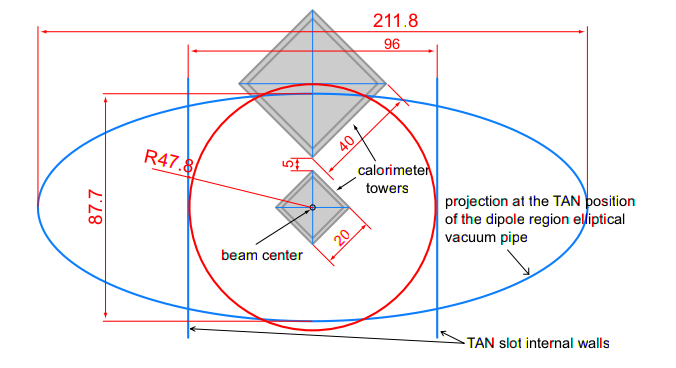
\includegraphics[scale=0.8]{lhcc1.png}
\caption{Schemat przedstawiający wymiary detektora (w mm). Źródło \cite{1}, s. 27.}\label{rys1}
\end{center}
\end{figure}

Każda wieża zbudowana jest z naprzemiennie umieszczonych warstw scyntylator-wolfram. 
Dodatkowo w każdej wieży umieszczone są 4 warstwy krzemowych
detektorów pozycjoczułych, których tutaj nie symulujemy. Grubości warstw scyntylatora oraz krzemowego detektora wynoszą 3 mm. Grubość
jednej warstwy wolframu to dwie drogi radiacyjne (Źr. \cite{2}). 
W głębszych częściach detektora, zgodnie z opisem (Źr. \cite{1}) umieszczono po dwie warstwy wolframu.
Zaimplementowany detektor przedstawiono na rysunku~\ref{rys2}.


\begin{figure}
\begin{center}
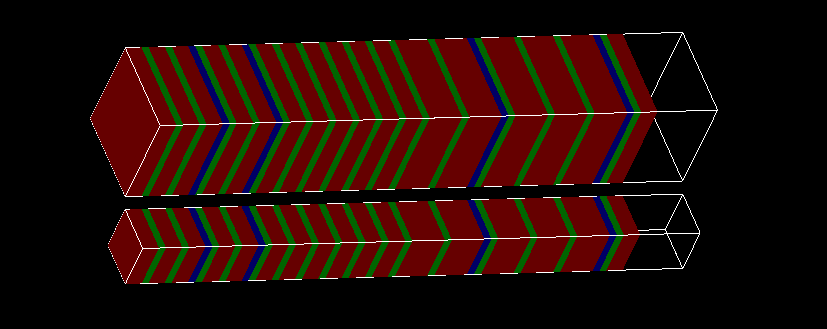
\includegraphics[width=0.45\linewidth]{moj_det.png}
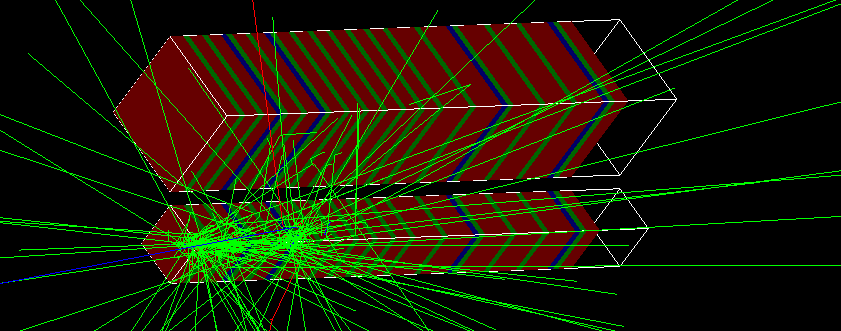
\includegraphics[width=0.45\linewidth]{lhcc3.png}
\caption{Rysunek przedstwaiający wizualizację zaimplementowanej geometrii detektora. Po prawej przedstawiono obrazowo powstającą 
kaskadę w detektorze dla fotonu o energii 1 GeV.}{\label{rys2}}
\end{center}
\end{figure}


W programie podczas symulacji może wystąpić przejście wtórnej cząstki pomiędzy wieżami. W rzeczywistości wieże są odseparowane. 
Zdecydowano się symulować każdą z wież oddzielnie, tak, aby wyeliminować ten efekt. Dodatkowym atutem jest tutaj nieznaczne skrócenie
czasu obliczeń oraz wyeliminowanie potrzeby implementacji dodatkowych elementów.

Symulację przeprowadzamy w każdym przypadku dla 1000 cząstek. Jest racjonalna wielkość, gdyż ze względu na duże energie wysyłanych
cząstek czas obliczeń jest znaczny.
%dodać zdjecie po implementacje 

\section*{Wyniki}

 Na wykresach przedstawiono sumaryczną energię zdeponowaną w danej warstwie scyntylatora.
W pierwszej kolejności wykonano symulacje dla każdej z cząstek (foton, neutron i pion $\pi^0$) przy zadanej energii 1 TeV. Wyniki dla obydwu wież 
przedstawiono na wykresach \ref{w1} (wieża centralna) oraz \ref{w2} (wieża boczna). 

Przy symulacji fotonu i pionu dla centralnej wieży energia zostaje zdeponowana głównie w pierwszej części detektora. 
Można zauważyć iż energia zdeponowana przez pion jest niższa niż dla fotonu. W symulacji dzieje się tak 
prawdopodobnie dlatego, gdyż użyliśmy cząstek o tej samej energii, a pion podczas lotu rozpada się na dwa fotony i nie każdy z nich trafia w centralny detektor.
 Natomiast dla neutronu obserwujemy znacznie niższą depozycję energii. 
 Z drugiej strony dla neutrony energia zostaje zdeponowana również w dalszych częściach detektora, co może umożliwić jego detekcję 
(np. ustawiając większą czułość w dalszych warstwach). 

W bocznej wieży rejestrujemy również fotony na które rozpada się pion. Natomiast nie rejestrujemy energii podczas symulacji fotonu, co może pozwolić 
na ich rozróżnienie w detektorze. W tej wieży w przypadku neutronu również rejestrujemy energię znacznie niższą niż w przypadku pionu.


\begin{figure}
\begin{center}
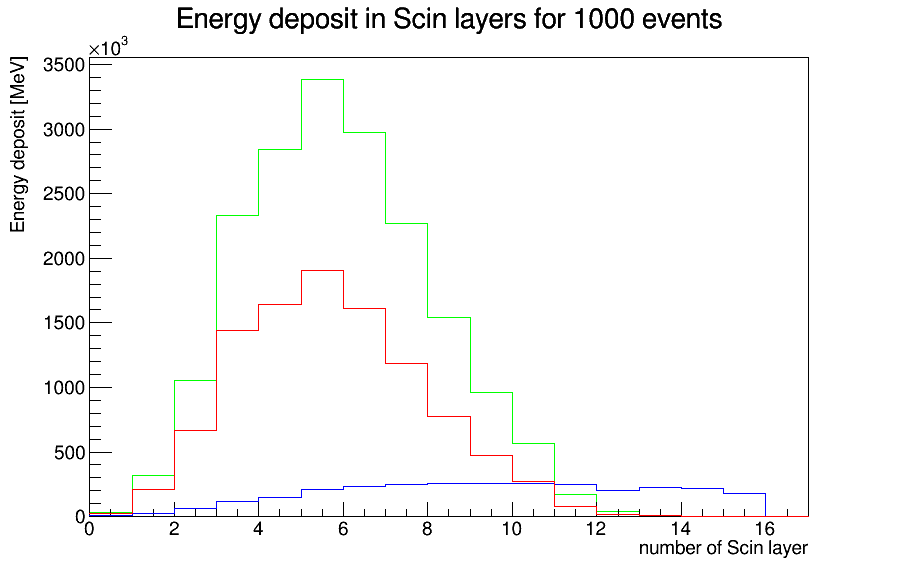
\includegraphics[scale=0.5]{cmp.png}
\caption{Na wykresie przedstawiono zdeponowaną energię w wieży centralnej w 
			kolejnych warstwach scyntylatora dla trzech cząstek: fotonu (kolor zielony), 
			neutronu (kolor niebieski), pionu (kolor czerwony).}\label{w1}
\end{center}
\end{figure}
\begin{figure}
\begin{center}
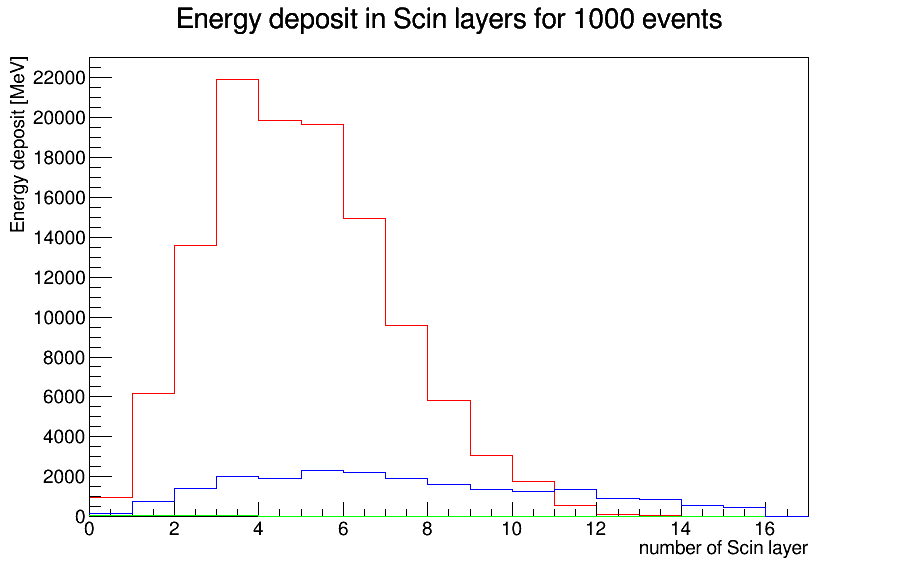
\includegraphics[scale=0.5]{scp.png}
\caption{Na wykresie przedstawiono zdeponowaną energię w wieży bocznej w 
			kolejnych warstwach scyntylatora dla trzech cząstek: fotonu (kolor zielony), 
			neutronu (kolor niebieski), pionu (kolor czerwony).}\label{w2}
\end{center}
\end{figure}


Następnie wykonano symulację dla różnych energii pierwotnego fotonu. Wynik przedstawiono na wykresie \ref{w3}. Widzimy, że im wyższa energia 
pierwotnego fotonu, tym większa energia zostaje zdeponowana. Obliczono całkowitą energię deponowaną w detoktorze (tabela \ref{t1}). 
Ilość zdeponowanej całkowitej energii zdeponowanej w wieży jest proporcjonalna do
energii wysłanego fotonu. 
\begin{table}
\caption{Całkowita energia zdeponowana w detoktorze w przeliczeniu na jeden foton.}\label{t1}
\centering
\begin{tabular}{c|c}
Energia pierwotnego fotonu $[$TeV$]$& Energia zdeponowana w detektorze $[$GeV$]$  \\ \hline
2 &36,9529 \\
1 &18,5066\\
0,5 &9,23262\\ 
0,1 & 1,79558 
\end{tabular}
\end{table}
\newpage
Przyjżyjmy się energi deponowanej przez pion. Całkowite zdeponowane energie przedstawiono w tabeli \ref{t2}. Stosunek tychże energii wnosi 0,054726. 
Zakładamy, że pion rozpada się na dwa fotony o równych energiach, w przybliżeniu 500 GeV. Z poprzednich symulacji wiemy jaka energia jest średnio deponowana
przez fotony o energiach 500 GeV. Porównyjąc ją z energiami uzyskanymi w symulacji pionów możemy sprawdzić jak dużo fotonów pochodzących z rozpadu pionu $\pi^0$
trafia w każdą z wież (tabela \ref{t2}). Widzimy, że w boczną wieżę trafia dużo mniej fotonów. W symulacji protony wysyłano z odległości 100 m. Fotony w 
rozpadzie pionu $\pi^0$ przy tak dużych energiach lecą pod małym kątem i możliwe, że przy większej odległości więcej fotonów trafi w boczną wieżę. Warto
zauważyć, że obliczenia te są przybliżone, a ilość energii deponowanej przez pojedynczy foton w każdej z wież może być inna, 
ze względu na różnice w ich wielkości. 
%Oznacza to iż około w pięciu na sto przypadkach pion rozpada się w taki sposób, że fotony trafiają w obie wieże detektora. Przyjmujemy, że fotony powstające
%pod odpowiednim kątem (czyli takim, aby trafiały w drugi detektor) są izotropowo rozłożone względem osi przechodzącej przez środek małej wieży. Powierzchnia 
%dużej wieży pokrywa około 9,5 \% \footnote{dokładniej 9.4917 \%}  powierzchni zajmowanej przez pierścień powstały przez obrót tejże wieży wokół wspomnianej osi. 
%Daje to około 57.7 \% \footnote{dokładniej 57.6567 \%} rozpadów w których produkty rozpadu pionu mogą trafić w obie wieże detektora. 
%\newline
%%%%%%%%%%%%%%%%%%%%%%%%%%%%%%%%%%%%%%%%%%%%%%%%%% \newpage dodane

\begin{figure}
\begin{center}
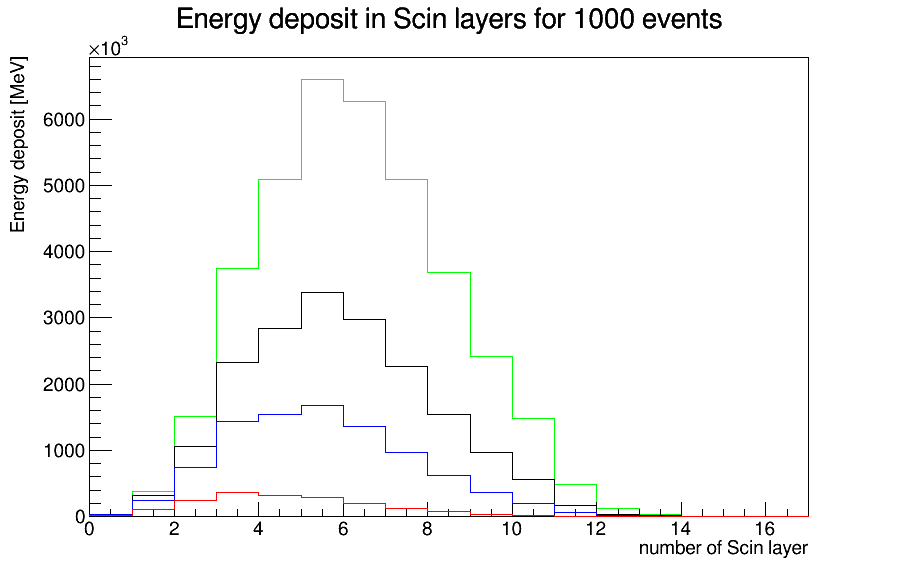
\includegraphics[scale=0.5]{gam.png}
\caption{Na wykresie przedstawiono zdeponowaną energię w wieży centralnej w 
			kolejnych warstwach scyntylatora dla różnych energii pierwotnego fotonu. Kolejno dla
			100 GeV (kolor czerwony), 500 GeV (kolor niebieski), 1 TeV (kolor czarny) oraz 2 TeV (kolor zielony).
			Wysokośc najwyższego odczytu rośnie wraz z energią. }\label{w3}
\end{center}
\end{figure}

\begin{table}
\caption{Energia deponownana oraz wyniki dla przypadku pionu dla 1000 eventów.}\label{t2}
\centering
\begin{tabular}{c|c}
& Całkowita zdeponowana energia $[$GeV$]$ \\ \hline  
centralna wieża & 1.03141 $\cdot 10^{4}$ \\ 
boczna wieża & 5.64450 $\cdot 10^{2}$ \\ \hline
& Obliczona ilość fotonów trawfiających w wieże \\ \hline
centralna wieża & 1117 \\
boczna wieża & 61 \\ \hline \hline
stosunek zdeponowanych energii & 0.054726 \\ 
\end{tabular}
\end{table}
%%%%%%%%%%%%%%%%%%%%%%%%%%%%%%%%%%%%%%%%%%%%%%%%%%%%%%%%%%%%%%%%%%%%%%%%%%%%%%%%%%
% the text
%%%%%%%%%%%%%%%%%%%%%%%%%%%%%%%%%%%%%%%%%%%%%%%%%%%%%%%%%%%%%%%%%%%%%%%%%%%%%%%%%%
\section*{Podsumowanie}
W projekcie zaimplementowano detektor złożony z dwuch kalorymetrów w postaci wież. Detektor ten jest przeznaczony do pomiaru 
cząstek neutralnych wyprodukowanych pod małymi kątami. Symulacja została przeprowadzona dla trzech różnych cząstek neutralnych: fotonu, neutronu oraz pionu $\pi^0$. 
Mierzono zdeponowaną energię w warstwach scyntylatorów zawartych w wieżach. W przypadku tychże cząstek znaleziono różnice w ddepozycie energii, które mogą umożliwić 
ich rozróżnienie. Sprawdzono również, że energia zdeponowana przez wpadający do kalorymetru foton jest proporcjonalna do jego energii. 


\begin{thebibliography}{99}
\bibitem{1} \url{http://home.agh.edu.pl/~leszekad/dydaktyka/wfiis_geant4_2015/lhcc-2006-004.pdf} Stan na 8.02.2015 r.
\bibitem{2} \url{http://pdg.lbl.gov/2011/AtomicNuclearProperties/HTML_PAGES/074.html} Stan na 5.01.2015 r.
\end{thebibliography}

\end{document}


